%%%%%% Design %%%%%%
\section{Design}

I dette afsnit beskrives systemets design. Systemet indeholder overordnet set de tre enheder drone, server og webapplikation samt en kommunikations protokol derimellem. Drone bruges til at overvåge og tage billeder, server står for håndtering af data, og webapplikation er systemets grænseflade til bruger. Mellem drone/server og webapplikation/server gøres brug af HTTP protokollen til kommunikation og udveksling af data.



\subsection{Drone}

Systemets bruger er ansvarlig for at lave flyveopsætninger, som indeholder informationer om det område drone skal overvåge.

Når drone tændes skal den løbende og uden menneskelig indblanding kontrollere om der er en ny flyveopsætning tilgængelig på server. Hvis der er en ny flyveopsætning tilgængelig hentes den, og en ny flyvning påbegyndes. 

Under flyvning flyver drone på egen hånd til de definerede GPS positioner. Afhængig af om bruger har valgt der skal tages billeder eller ej, tager dronen billeder som via mobilt netværk sendes til server. 
Under flyvning kontrollerer drone løbende egen GPS position, flyvehøjde og flyveretning. Dette gør dronen for løbende at kunne tilpasse flyvehøjde og orientering og for at kunne sende information om nuværende GPS position til server.

På figur \ref{fig:class_drone} vises et simplificeret klasse diagram for drone. I det viste klassediagram vises softwareklasser og deres indbyrdes forhold. For yderlige information om de enkelte klasser, deres metoder og deres ansvarsområder henvises til logical view [x]

\begin{figure}[H]
\centering
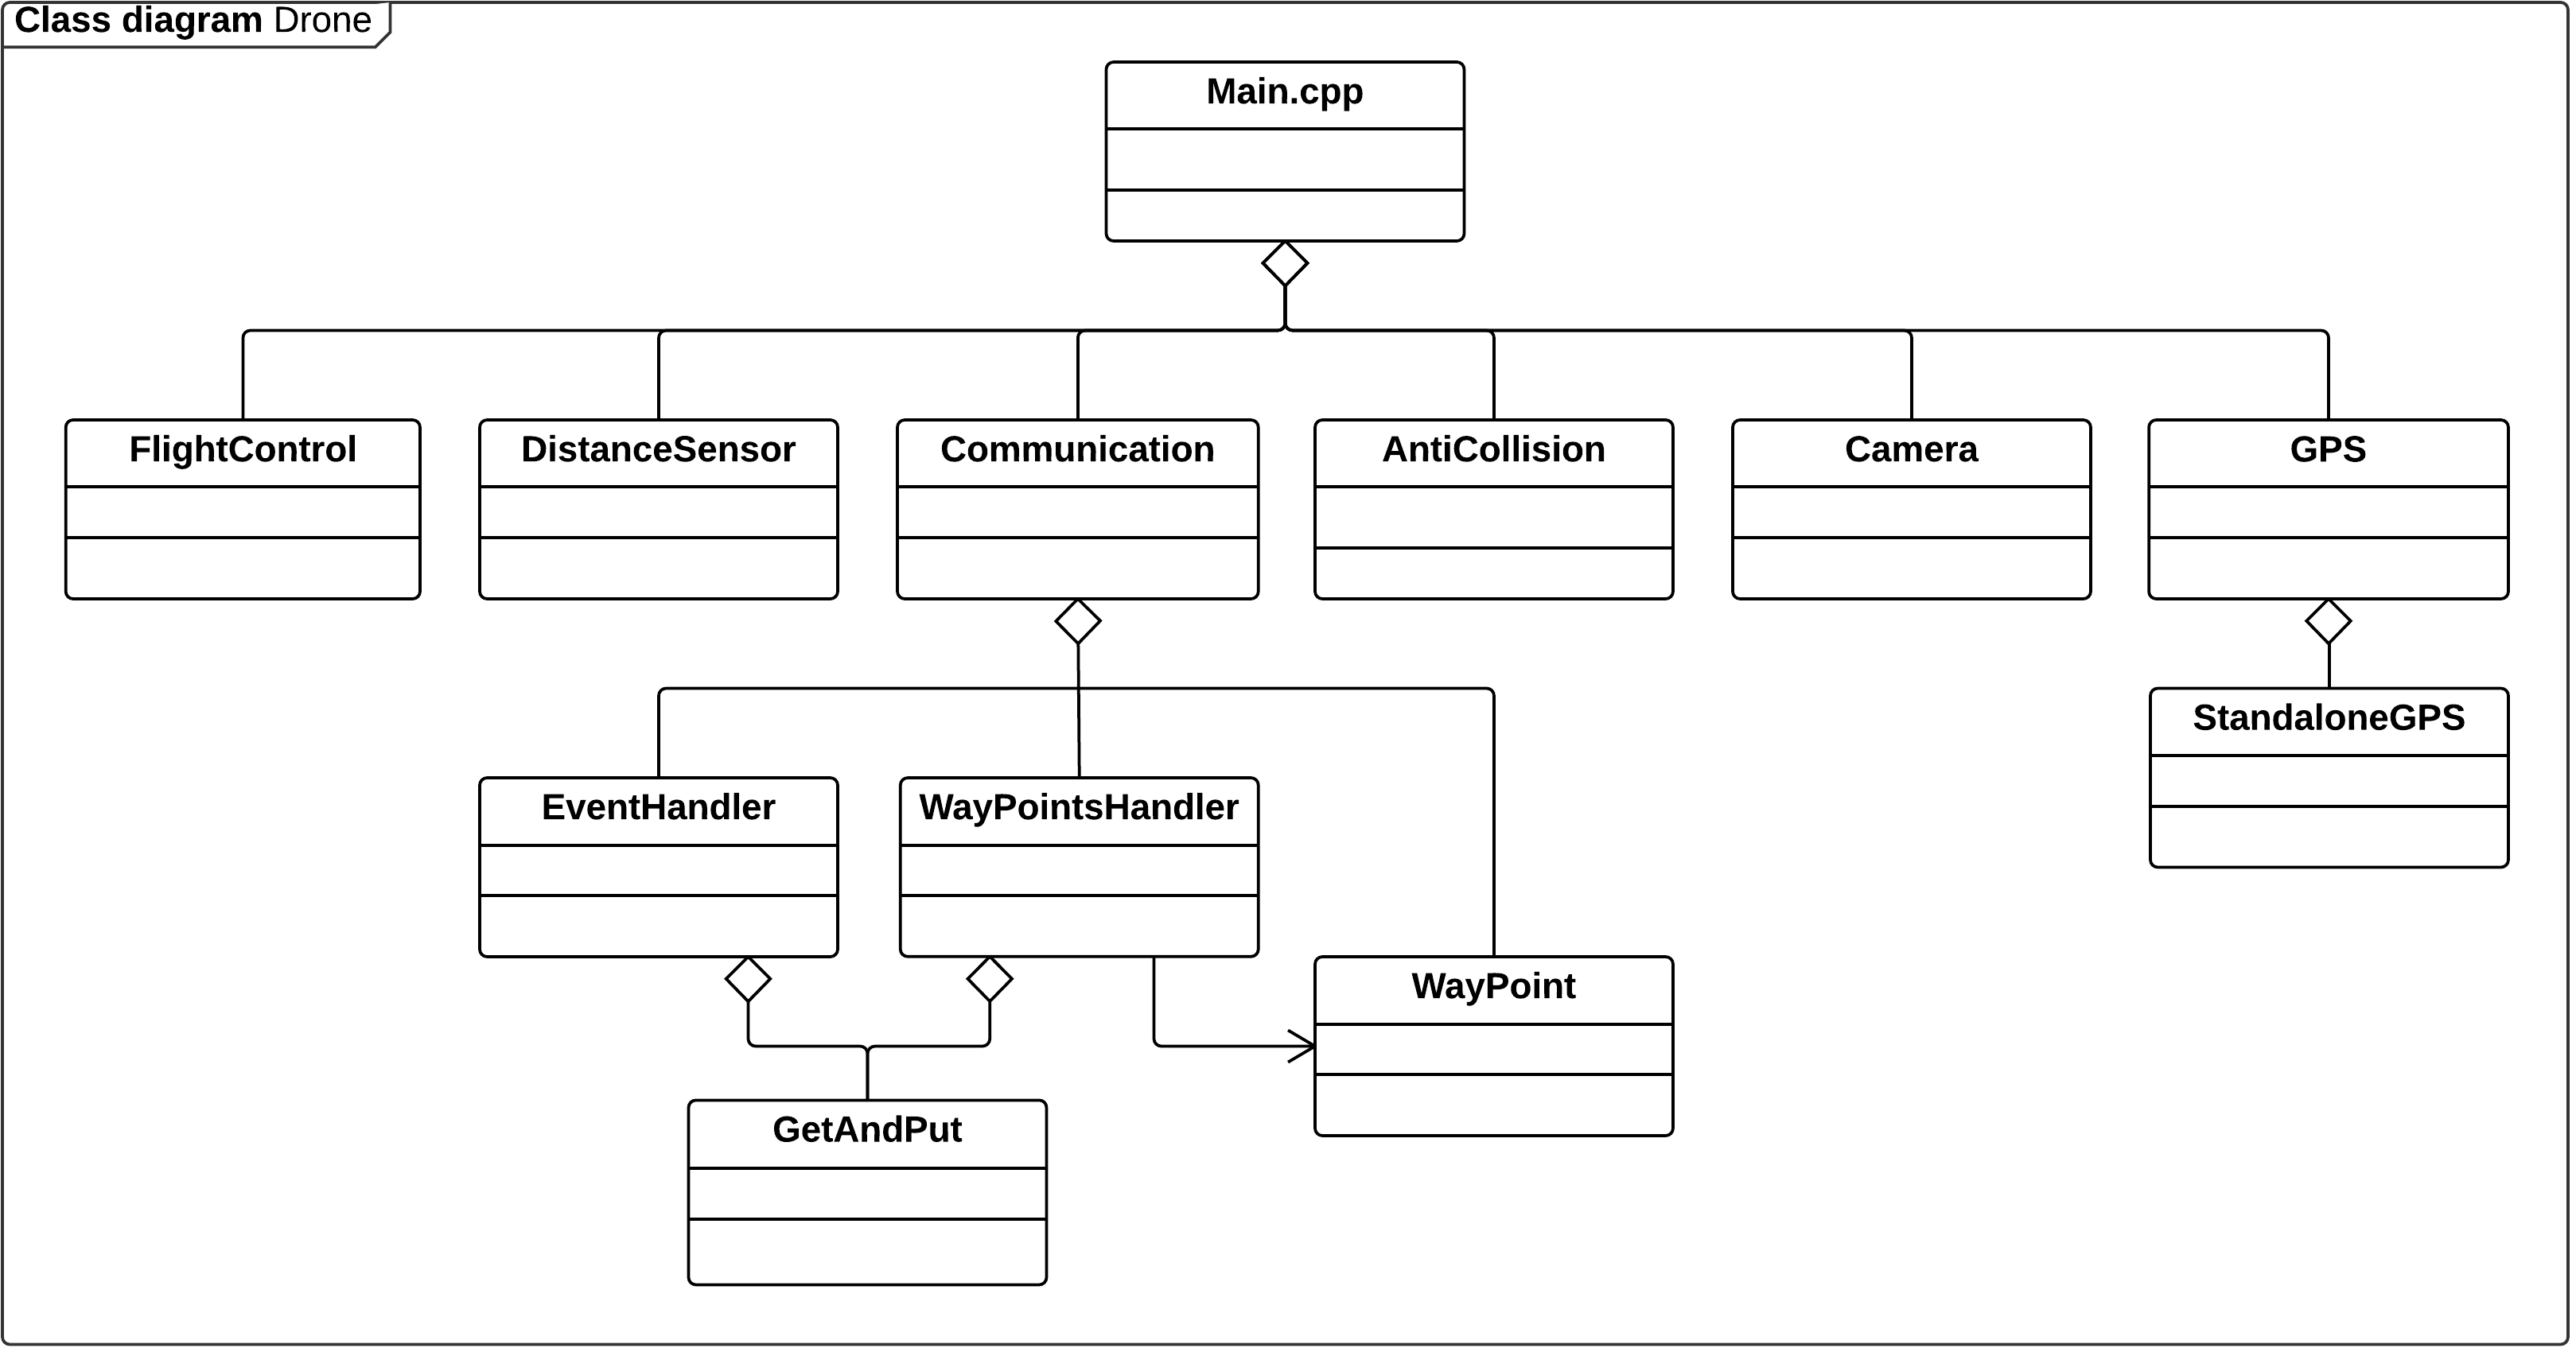
\includegraphics[width=1\textwidth]{Billeder/Design_Class_drone.png}
\vspace{-0.5cm}
\caption{Klassediagram drone}
\label{fig:class_drone}
\end{figure}


\newpage 

\subsection{Server}

Server består af SQLite database med et tilhørende REST API. I SQLite databasen gemmes og hentes løbende information om systemets brugere, samt information om flyveopsætninger, flyveruter og billeder.  

Server er en passiv enhed, som er ansvarlig for håndtering af systemets data. Server tager aldrig initiativ til udveksling af data, den står i stedet og venter på at blive igangsat af enten drone eller webapplikation.

For systemets bruger kan det se ud som om udveksling af data og information går direkte fra webapplikation til drone eller omvendt. Men reelt set er webapplikation og drone aldrig i direkte kontakt med hinanden. I stedet går al kommunikation til og fra server via HTTP protokollen. 

På figur \ref{fig:deployment_diagram} ses et deployment diagram, der viser hvordan drone og webapplikation kommunikerer med server for at hente og gemme information. For yderlige information om server og tilhørende SQLite database henvises til data view [x].

\begin{figure}[H]
\centering
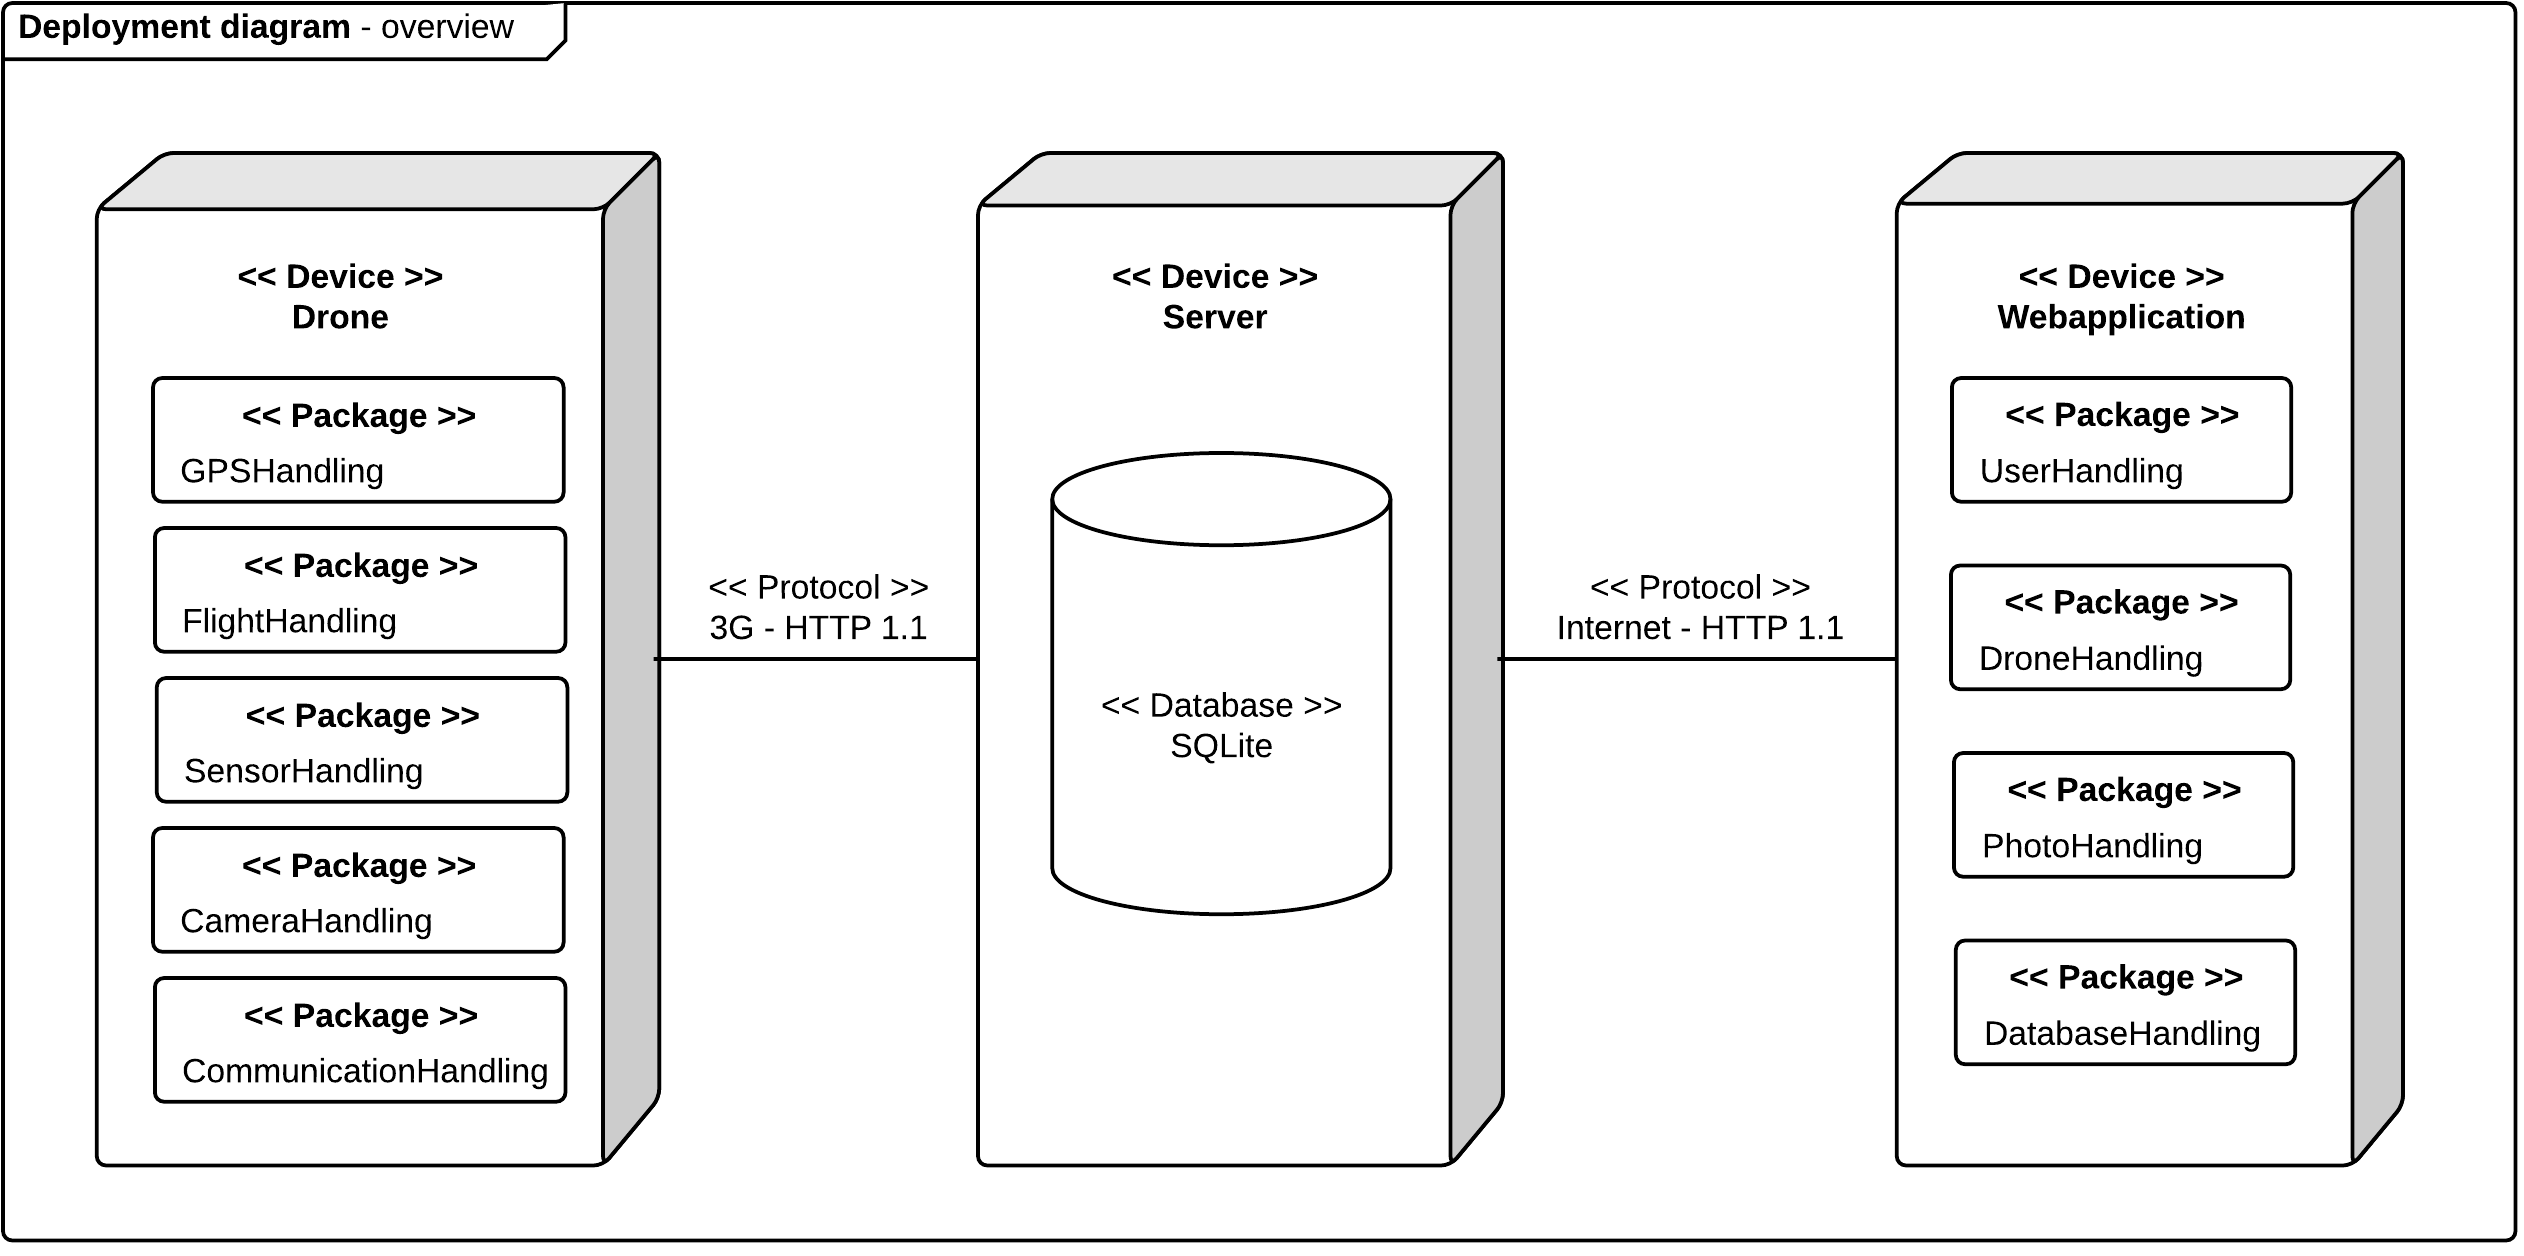
\includegraphics[width=1\textwidth]{Billeder/deployment_overview.png}
\vspace{-0.5cm}
\caption{Deployment diagram}
\label{fig:deployment_diagram}
\end{figure}
 
\newpage


\subsection{Webapplikation}

Webapplikationen fungerer som grænseflade til systemets bruger. Da det ikke ønskes at alle og enhver kan tilgå webapplikationen, skal bruger logge ind før webapplikations funktionalitet kan benyttes. 

Via webapplikationen kan bruger lave nye flyveopsætninger samt monitorere data og information fra tidligere flyvninger. Da det ikke er muligt at rette eller stoppe en aktuel flyvning, skal bruger være opmærksom på hvordan en ny flyveopsætning indstilles. 

Mellem server og webapplikation laves en socket connection. Dette betyder at indholdet af webapplikationen opdateres hver gang der der tilføjes eller ændres i eksisterende data på serverens SQLite database. Yderlige information om webapplikations diagrammer findes i logical view [X] og implementation view [X].


\subsection{HTTP protokol}

Den kommunikationsprotokol der bruges til at sende og modtage data fra server ønskes benyttet af både webapplikation og drone. Da der kun skal laves et interface til server, hvis drone og webapplikation benytter samme protokol.

Webapplikationen kan benytte stort set alle kommunikations protokoller, mens 3G/GPS modulet kun kan benytte et begrænset antal.

Det vælges at benytte HTTP protokollen, da 3G/GPS modulet understøtter denne protokol og fordi protokollen er blandt de mest anvendte protokoller til kommunikation mellem webapplikationer og servere.

Ønskes yderlige viden om HTTP protokollen henvises til W3 [x], mens der henvis til deployment view [X], hvis der ønskes mere viden om brug af protokollen. 
